\section{Finding 11 - No Encryption for Webserver on Port 80}
%center under chapter title a one row table with 6 coloumns and no borders
\vspace*{-0,3cm}
\begin{center}
    \begin{tabular}{c c c c}
        \textbf{Classification:} & Misconfiguration & \textbf{Severity:} & \textbf{\textcolor{red}{High}}  
        \end{tabular}
\end{center}

A portscan of the \ac{DUT} revealed that the Webserver on port 80 is not encrypted.

\subsection{Finding Impact}
All of the traffic between the client and the Webserver is unencrypted. This allows an attacker to intercept the traffic and read the data.

\subsection{Finding Details}
The following screenshot shows an excerpt of a wireshark capture. This is how an atacker could intercept the traffic: 
\begin{figure}[h]
    \centering
    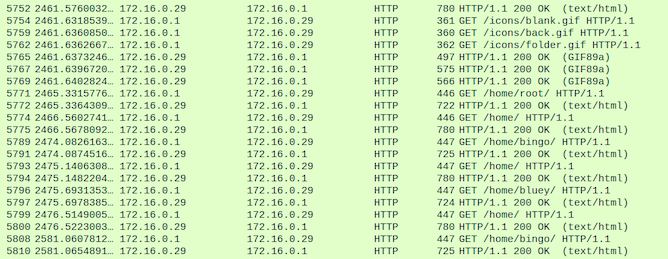
\includegraphics[width=0.8\textwidth]{img/no_encryption_port_80.png}
    \caption{Screenshot of Wireshark}
    \label{fig:fin11}
\end{figure}

Following is the output of the portscan which shows that the Webserver on port 80 uses http:
\begin{lstlisting}[language=bash]
$ nmap -A 172.16.0.29
    
Starting Nmap 7.93 ( https: //nmap.org ) at 2023-03-06 09:30 CET
Nmap scan report for 172.16.0.29
Host is up (0.00051s latency).
    
PORT STATE SERVICE VERSION
80/tcp open http Apache httpd 2.4.54 ((Debian))
\end{lstlisting}


\subsection{Evaluation of Results}
\begin{center}
    \begin{tabular}{cccc}
    \textbf{Effort to Fix:} & &\ \textbf{\textcolor{orange}{Medium}}\
    \end{tabular}
\end{center}
Traffic between clients and the webserver should be encrypted. This can be done by using a certificate for the webserver. This certificate should be signed by a trusted \ac{CA}. This can be done by using a certificate from a \ac{CA} like \href{https://letsencrypt.org/}{Let's Encrypt}.
